\section{Experiment and Analysis}
\label{sec:experiment}

In this section, we introduce the measurements experiments setup and 
evaluate the process of probabilistic forecasting of channel state.

% Subsec Experiment design
\subsection{Measurements}
\label{subsec:measurements}

% 24 hours measurement introduction
We perform measurements in neighborhoods, campus, downtown bussiness office and 
urban bussiness office for 24 hours on weekdays. 
The locations we chosen for measurements are shown in Fig.~\ref{fig:measurement_map}.

\begin{figure}
\vspace{-0.0in}
\centering
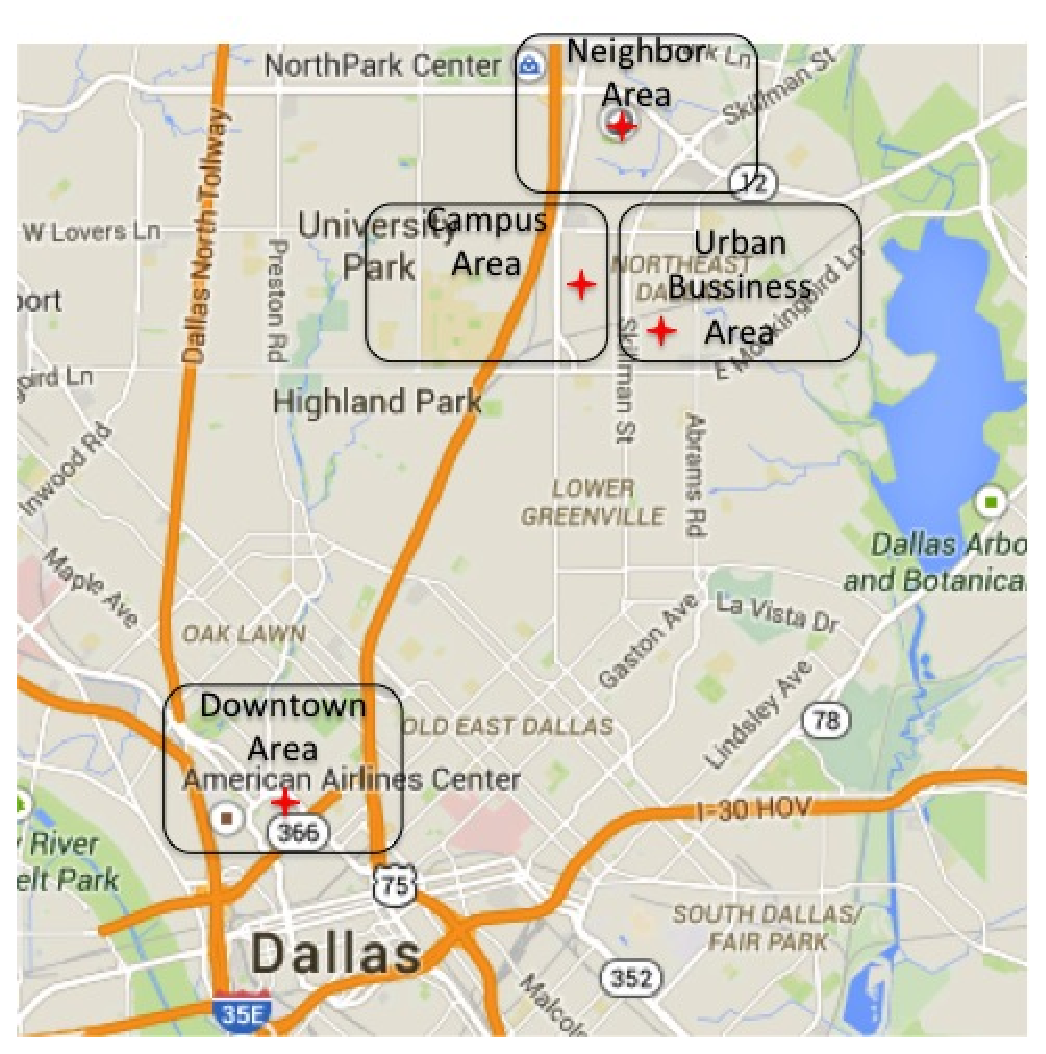
\includegraphics[width=84mm]{figures/measurements_map}
\vspace{-0.1in}
\caption{Long Term Measurements Locations}
\label{fig:measurement_map}
\vspace{-0.1in}
\end{figure}




% Experiment equipment
We employ a Rohde \& Schwarz FSH8 portable spectrum works from 100 KHz to 8 GHz. 
The portable spectrum analyzer is controlled by a Python script on a laptop to measure 
the received signal strength.
% Data normalize 
To the best of our knowledge, there is no readily available mobile, multiband antenna from
450 MHz to 5.2 GHz on the market. Thus, we use a 700-MHz mobile antenna to perform in-field
measurements. We then normalize the mobile antenna performance across bands with indoor 
experimentation. To do so, we use a Universal Software Radio Peripheral (USRP) N210 to 
generate signals at 450 MHz, 800 MHz, and 2.4 GHz. We feed the USRP signals directly
to a spectrum analyzer and adjust the configuration of USRP to make the received signal 
strength the same as the 5.2 GHz signal from Gateworks 2358 with a XR5 radio. Then, we connect 
the signal source to a fixed multiband antenna (QT 400 Quad Ridge Horn Antenna) and measure the
received signal at a fixed distance with the 700 MHz antenna and antennas for different bands
to obtain the antenna loss for each band. We adjust the received signal strength
collected via the 700-MHz mobile antenna according to the normalization.

% Introduce how to calculate the capacity
% Explain multiband and activity level
When wireless devices operate in WiFi bands, the channel separation is relatively 
small (e.g., 5 MHz for the 2.4 GHz band). As a result, many works assume that
the propagation characteristics across channels are similar. However, with the
large frequency differences between WiFi and white space bands (e.g., multiple GHz),
propagation becomes a key factor in the deployment of wireless networks with both bands.
Here, a frequency band is defined as a group of channels which have
little frequency separation, meaning they have similar propagation characteristics.
In this work, we consider the diverse propagation and activity characteristics
for four total frequency bands: 450 MHz, 800 MHz, 2.4 GHz, and 5.2 GHz.
We refer to the two former frequency bands as white space bands and
the two latter frequency bands as WiFi bands.
The differences in propagation and spectrum utilization create opportunities
for the joint use of white space and WiFi bands in wireless access networks according
to the environmental characteristics (e.g., urban or rural and downtown or residential)
of the deployment location.


For spectrum utility and resulting channel availability, 
we split the measurements every 30 minutes of each band.  We define the percentage of sensing 
samples ($S_\theta$) above an interference threshold ($\theta$) over the total samples ($S$) in 
a time unit as the activity level ($A$) of inter-network interference:
\begin{equation}
\label{eq:actdef}
A=\frac{S_\theta}{S_a}
\end{equation}
The capacity of a clean channel is denoted by $C$. With the protocol model, the capacity 
of a channel with inter-network interference $C_r$ could be represented as 
the remaining free time of the channel capacity according to: 
\begin{equation}
\label{eq:intercap}
C_r=C*(1-\bar{A})
\end{equation}


% Need to discuss the \mu mapping with these measurements stuff


\begin{table*}
\centering % centering table 
\begin{tabular}{|l|c|c|c|c|c|c|c|c|c|c|c|c|c|c|} % creating 13 columns 
\hline %\hline % inserting double-line 
%Bands     & \multicolumn{3}{c|}{Dallas} & \multicolumn{3}{c|}{Weatherford} & \multicolumn{3}{c|}{Millsap} \\% [0.5ex]
%\hline % inserts single-line 
% Entering 1st row 
%Area Type & Downtown & Residential & Suburban & Downtown &  Residential & Sparse & Downtown & Residential & Sparse \\ % [0.5ex]
\hline % inserts single-line 
\multirow{8}{*}{Downtown}	
&\multirow{2}{*}{400 MHz}	
&0:00-11:00 &  23.17 &  23.69 &  23.45 &  22.83 &  23.24 &  23.43&  23.48 &  23.74&  23.69 &  23.36&  23.29 &  23.00 \\ 	
\cline{3-15}	
&&12:00-23:00&  22.85 &  22.81 &  23.62 &  23.74 &  23.14 &  23.48&  23.38 &  22.52&  22.04 &  22.59&  22.59 &  22.42 \\ 	
\cline{2-15}	
&\multirow{2}{*}{800 MHz}	
&0:00-11:00 &  12.63 &  13.20 &  13.08 &  12.94 &  11.55 &  11.48&  11.60 &  11.38&  11.86 &  11.72&  10.47 &  10.32 \\ 	
\cline{3-15}	
&&12:00-23:00&  12.00 &  11.86 &  10.71 &  11.93 &  12.72 &  12.36&  11.48 &  11.43&  11.72 &  11.60&  11.72 &  11.91 \\ 	
\cline{2-15}	
&\multirow{2}{*}{2.4 GHz}	
&0:00-11:00 &  29.04 &  28.66 &  27.29 &  28.15 &  27.89 &  27.72&  28.18 &  27.38&  28.18 &  27.74&  28.15 &  27.96 \\ 	
\cline{3-15}	
&&12:00-23:00&  27.96 &  29.14 &  28.97 &  28.20 &  28.80 &  29.57&  29.02 &  27.72&  27.70 &  27.77&  29.21 &  28.42 \\ 	
\cline{2-15}	
&\multirow{2}{*}{5.2 GHz}	
&0:00-11:00 &  25.41 &  25.29 &  26.32 &  26.49 &  27.23 &  27.28&  26.99 &  26.27&  25.36 &  26.13&  25.81 &  24.88 \\ 	
\cline{3-15}	
&&12:00-23:00&  26.92 &  26.49 &  26.41 &  27.11 &  25.67 &  26.53&  26.73 &  26.97&  26.32 &  25.79&  27.57 &  26.65 \\ 	
\hline	
\multirow{8}{*}{Urban}	
&\multirow{2}{*}{400 MHz}	
&0:00-11:00 &  22.09 &  21.27 &  22.28 &  22.47 &  21.65 &  21.68&  22.37 &  22.16&  23.12 &  22.73&  22.01 &  22.54 \\ 	
\cline{3-15}	
&&12:00-23:00&  21.80 &  20.86 &  21.80 &  22.54 &  22.35 &  22.61&  22.45 &  21.58&  22.18 &  23.09&  22.11 &  22.09 \\ 	
\cline{2-15}	
&\multirow{2}{*}{800 MHz}	
&0:00-11:00 &  12.99 &  12.44 &  12.08 &  12.32 &  11.60 &  11.60&  12.48 &  12.10&  11.14 &  11.55&  11.98 &  11.12 \\ 	
\cline{3-15}	
&&12:00-23:00&  11.88 &  12.27 &  12.36 &  12.05 &  12.15 &  14.00&  13.32 &  12.29&  11.38 &  11.55&  12.92 &  13.16 \\ 	
\cline{2-15}	
&\multirow{2}{*}{2.4 GHz}	
&0:00-11:00 &  29.08 &  29.15 &  29.49 &  28.93 &  29.01 &  28.86&  28.84 &  29.53&  29.03 &  28.74&  29.89 &  29.15 \\ 	
\cline{3-15}	
&&12:00-23:00&  28.60 &  29.61 &  29.44 &  28.55 &  28.05 &  28.62&  28.74 &  28.93&  28.26 &  27.73&  28.19 &  29.85 \\ 	
\cline{2-15}	
&\multirow{2}{*}{5.2 GHz}	
&0:00-11:00 &  27.21 &  27.11 &  26.20 &  25.77 &  26.70 &  26.17&  25.67 &  26.10&  25.77 &  25.41&  26.05 &  26.34 \\ 	
\cline{3-15}	
&&12:00-23:00&  26.17 &  26.03 &  25.19 &  26.41 &  26.80 &  25.17&  26.08 &  25.60&  26.44 &  26.58&  25.50 &  25.45 \\ 	
\hline	
\multirow{8}{*}{Campus}	
&\multirow{2}{*}{400 MHz}	
&0:00-11:00 &  20.29 &  21.56 &  21.41 &  22.52 &  23.12 &  21.97&  21.65 &  21.63&  21.87 &  21.22&  21.17 &  21.39 \\ 	
\cline{3-15}	
&&12:00-23:00&  22.33 &  22.88 &  22.28 &  21.65 &  22.49 &  22.16&  21.32 &  22.35&  21.56 &  21.75&  21.75 &  20.45 \\ 	
\cline{2-15}	
&\multirow{2}{*}{800 MHz}	
&0:00-11:00 &  11.98 &  12.20 &  12.68 &  12.03 &  11.52 &  11.19&  11.96 &  12.94&  11.52 &  11.93&  12.44 &  10.95 \\ 	
\cline{3-15}	
&&12:00-23:00&  11.26 &  11.62 &  12.12 &  12.70 &  12.34 &  11.62&  11.57 &  12.17&  11.55 &  12.08&  11.88 &  11.98 \\ 	
\cline{2-15}	
&\multirow{2}{*}{2.4 GHz}	
&0:00-11:00 &  26.10 &  25.91 &  28.02 &  26.61 &  27.90 &  27.09&  27.01 &  27.21&  26.99 &  26.75&  25.69 &  26.46 \\ 	
\cline{3-15}	
&&12:00-23:00&  26.58 &  27.23 &  26.92 &  26.29 &  26.10 &  26.13&  26.25 &  25.53&  25.79 &  25.84&  26.13 &  26.46 \\ 	
\cline{2-15}	
&\multirow{2}{*}{5.2 GHz}	
&0:00-11:00 &  26.68 &  26.05 &  25.12 &  25.93 &  25.36 &  25.79&  26.03 &  26.73&  25.89 &  25.26&  25.81 &  25.50 \\ 	
\cline{3-15}	
&&12:00-23:00&  25.19 &  25.60 &  24.52 &  25.00 &  26.08 &  26.17&  26.85 &  26.53&  26.10 &  25.53&  25.89 &  25.31 \\ 	
\hline	
\multirow{8}{*}{Neighborhoods}	
&\multirow{2}{*}{400 MHz}	
&0:00-11:00 &  23.17 &  24.35 &  23.82 &  23.75 &  23.44 &  22.76&  24.08 &  25.26&  24.54 &  23.87&  23.82 &  23.70 \\ 	
\cline{3-15}	
&&12:00-23:00&  23.48 &  22.67 &  23.53 &  23.48 &  23.99 &  24.49&  23.99 &  22.98&  22.86 &  23.03&  23.89 &  23.63 \\ 	
\cline{2-15}	
&\multirow{2}{*}{800 MHz}	
&0:00-11:00 &  15.72 &  16.30 &  16.33 &  15.72 &  16.54 &  14.48&  14.62 &  14.48&  15.68 &  15.03&  15.60 &  16.33 \\ 	
\cline{3-15}	
&&12:00-23:00&  15.72 &  14.74 &  14.74 &  14.38 &  15.41 &  15.00&  15.84 &  16.25&  14.84 &  14.69&  15.51 &  14.93 \\ 	
\cline{2-15}	
&\multirow{2}{*}{2.4 GHz}	
&0:00-11:00 &  26.49 &  26.37 &  26.22 &  26.03 &  24.97 &  27.16&  27.76 &  26.56&  26.05 &  26.22&  25.74 &  27.18 \\ 	
\cline{3-15}	
&&12:00-23:00&  27.01 &  26.34 &  25.79 &  25.48 &  26.53 &  26.29&  25.33 &  25.86&  26.92 &  25.98&  25.48 &  27.66 \\ 	
\cline{2-15}	
&\multirow{2}{*}{5.2 GHz}	
&0:00-11:00 &  25.93 &  26.27 &  25.07 &  25.67 &  26.77 &  26.80&  27.52 &  25.38&  25.55 &  25.86&  25.62 &  26.13 \\ 	
\cline{3-15}	
&&12:00-23:00&  25.29 &  26.49 &  26.70 &  26.77 &  25.31 &  24.59&  24.78 &  25.91&  25.67 &  24.73&  24.73 &  25.21 \\ 	
\hline	
\end{tabular}    
\caption{Activity Level in Multiple Locations (To Be removed)} % title name of the table 
\label{tab:activitymeasurement}    
\vspace{-0.3in}
\end{table*}    












% Mobility pattern measurements
White space band is in advantage to adapt user moving in the area. To identify the user mobility pattern, we leverage 
the data from WiEye database and find the user locations across time.
% WiEye introduction
WiEye application created for the data collection is currently available for download and usage via the Google Android 
Market under the name WiEye. The application offers WiFi access points connection quality in both graphical and tabular 
form. All data collection is done in the background, either continuously while the user is running the application or 
periodically if the user has opted in to background data collection to SMU research. 
The data collected has been approved by the Southern Methodist UniversityInstitutional Review Board, a human subjects 
research committee,ensuring that all ethical precautions have been taken in collectingdata from the users of our 
application.
The dataset we chosen from the WiEye database is measured in the weekdays of around Dallas areas as shown in Fig~\ref{fig:measurementsmap}.


The distribution of the users are shown in Fig~\ref{fig:wieyeprocess}

\begin{figure}
\vspace{-0.0in}
\centering
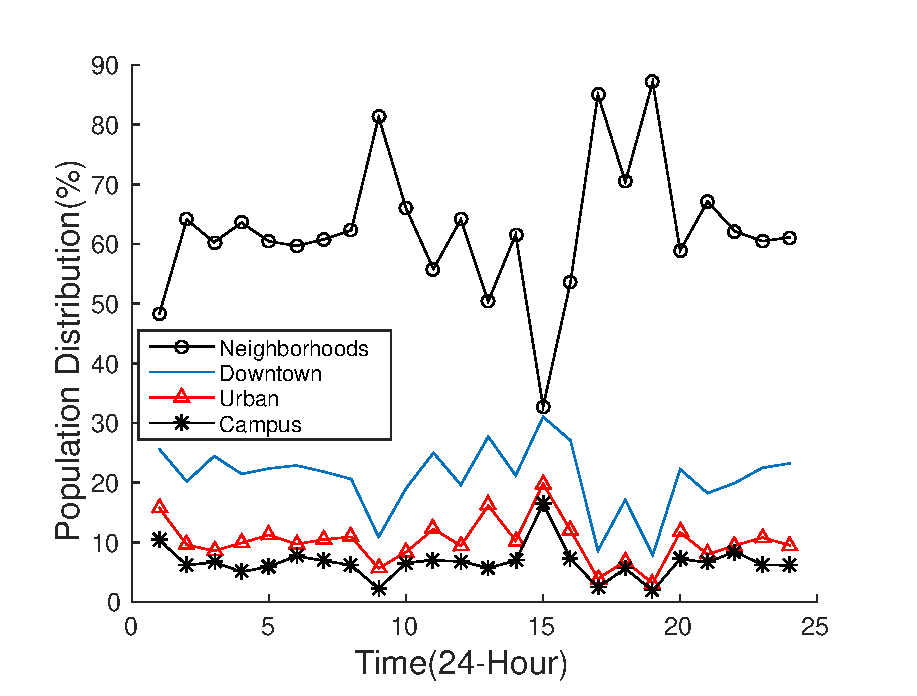
\includegraphics[width=84mm]{figures/wieyeprocess}
\vspace{-0.1in}
\caption{User Distribution across Time}
\label{fig:wieyeprocess}
\vspace{-0.1in}
\end{figure}

% Insert the table with hour vs user number & percentage



\subsection{Experiment Setup}
\label{subsec:experimentsetup}

% Virtual city setup
In this subsection, we apply our GSR algorithm with the measurements in a virtual city to investigate 
white space band impacts on power consumption. 
The virtual city include a downtown area, a school campus area, two urban bussiness areas and three 
neighborhood areas. All the areas are in the same size fit for a single WiFi cell. 
The white space channels has more than 3 times propagation range than WiFi channels cover 
all the WiFi cells.
We assume residents of the city is a constant number. 
People move from the neighborhoods to the business area and campus in the morning and back in the late 
afternoon. We assume in a certain weekday all the users are at home. 
%FIXME insert the data of wieye results




%The users start to move at 6:00  with 12\% per half hour until 
%9:30 . the remaining 16\% of users will stay at home in the day time. 
%The users are distributed to the downtown bussiness, urban and school campus areas with ratio 4:3:2.
%In the late afternoon, users starts to go home 
%with a rate 16\% of total users per half hour from 17:00 to 19:00 and 
%the ratio among the area types are 5:4:3.
%The other 3\% users will staty 
%in the downtown bussiness area and 1\% stay in urban bussiness area till midnight. 

%To be clear, we list the population distribution setup of the four areas in Table~\ref{tab:populationsetup}


% Time population, user traffic demand and radios capacity setup
The transmit power of radios are equal and with the same clean channel capacity. 
The standby power consumption of a radio is 50 watt and transmit power is 0.5 watt per Mbps.
We lookup population distribution from the US census 2010 to calculate the users in the 
virtual city. We set the demand requested per user as 0.5 Mbps and assume 30\% of the users will 
activate their device (ie. the take rate is 30) from 6:00 to 24:00. From 24:00 to 6:00, 5\% of 
the users device keep working. 
%  Fixme Time of traffic distribution



% Time population, user traffic demand and radios capacity setup
The transmit power of radios are equal and with the same clean channel capacity. 
The standby power consumption of a radio is 50 watt and transmit power is 0.5 watt per Mbps.
We lookup population distribution from the US census 2010 to calculate the users in the 
virtual city. We set the demand requested per user as 1 Mbps and assume 30\% of the users will 
activate their device (ie. the take rate is 30). 

% Move form homr to school
% night move home


% percentage of resident use the network in day time and night











\subsection{Results and Analysis}
\label{subsec:results}



% Investigate time

\begin{figure}
\vspace{-0.0in}
\centering
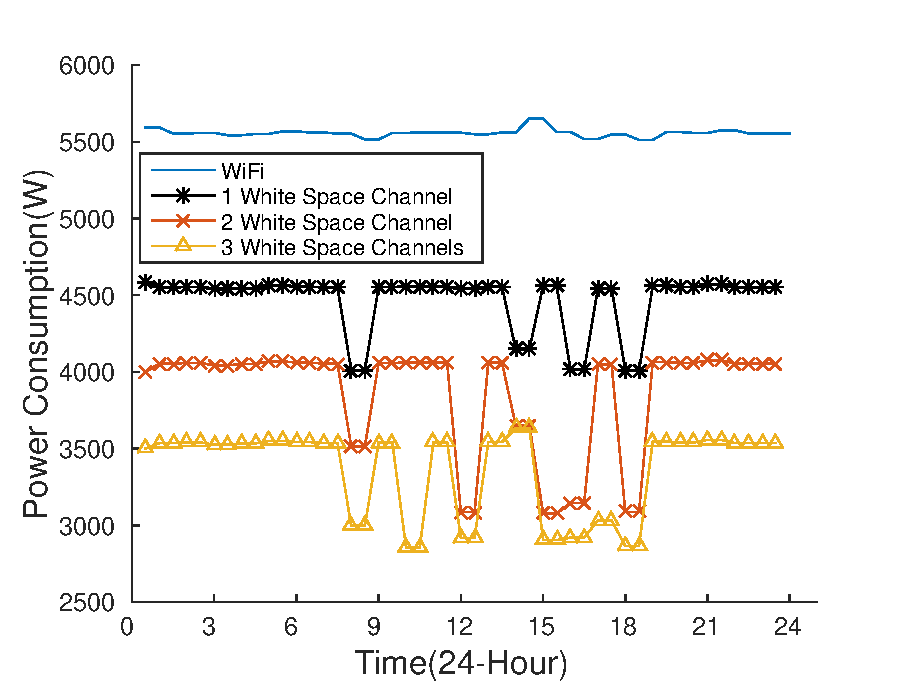
\includegraphics[width=84mm]{figures/timevary}
\vspace{-0.1in}
\caption{Power Consumption across Time}
\label{fig:timevary}
\vspace{-0.1in}
\end{figure}


% Robust



% Different cities



% forget the last one, check the notes monday


% Delay variation
\begin{figure}
\vspace{-0.0in}
\centering
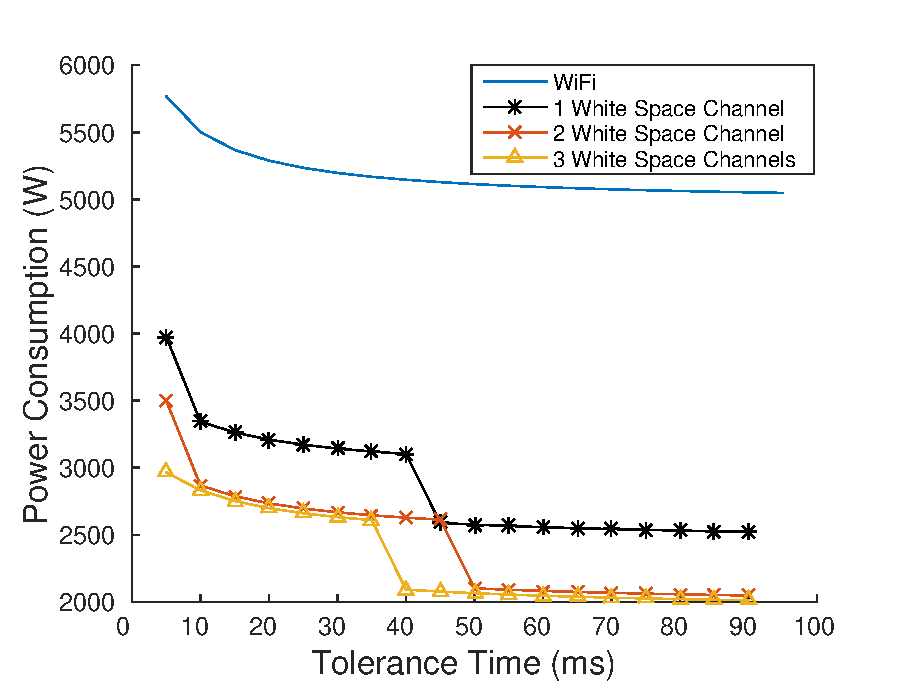
\includegraphics[width=84mm]{figures/delay_vary}
\vspace{-0.1in}
\caption{Power Consumption across Delay Tolerance}
\label{fig:delayvary}
\vspace{-0.1in}
\end{figure}


% Fit for long delay tolerance,if small delay require more resource



% Not sentivitv to population? need more resultes
\begin{figure}
\vspace{-0.0in}
\centering
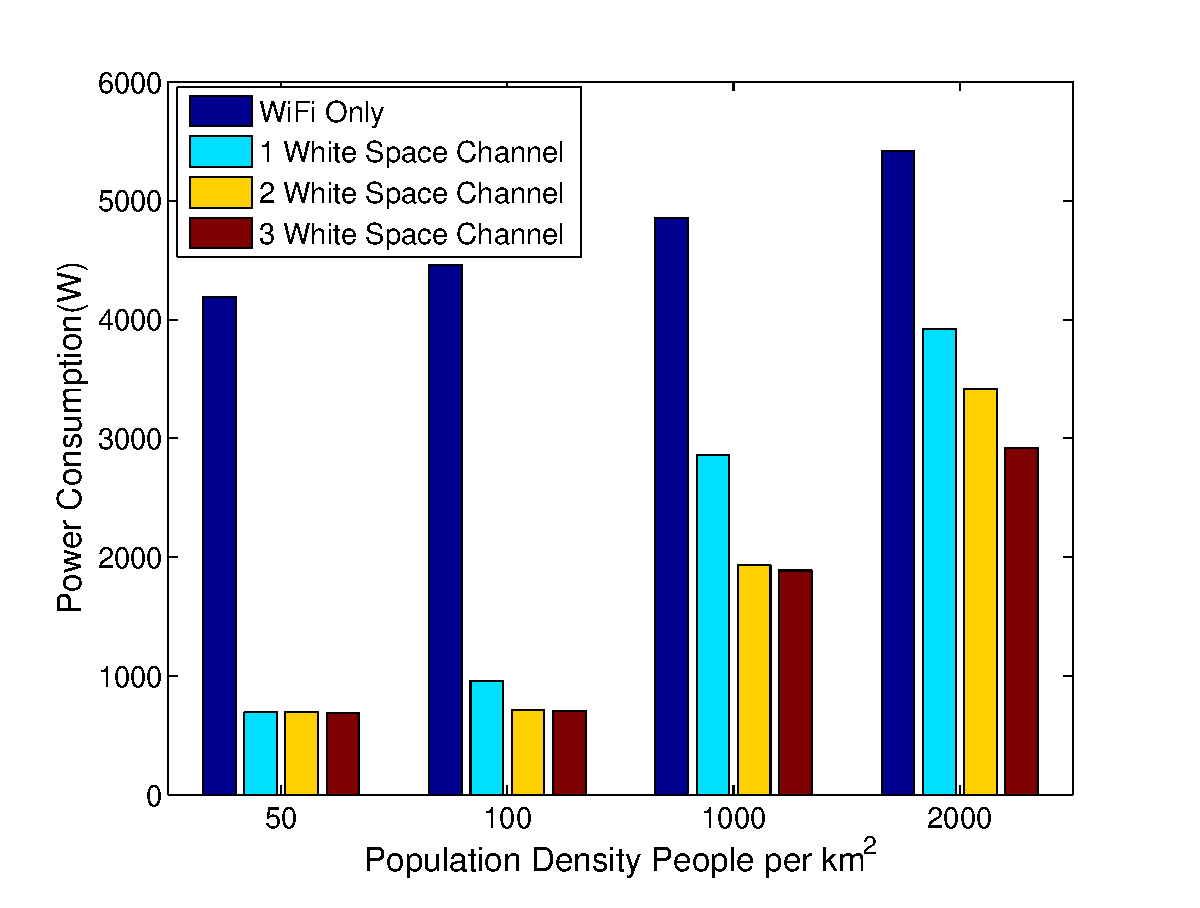
\includegraphics[width=84mm]{figures/populationvary}
\vspace{-0.1in}
\caption{Power Consumption across Population Distribution}
\label{fig:delayvary}
\vspace{-0.1in}
\end{figure}



